\documentclass[11pt]{article}

% --- packages ---
\usepackage[margin=1in]{geometry}
\usepackage{amsmath,amssymb,amsfonts}
\usepackage{booktabs}
\usepackage{graphicx}
\usepackage{hyperref}
\usepackage{xcolor}
\usepackage{multirow}
\usepackage{float}
\usepackage[numbers]{natbib}
\usepackage{algorithm}
\usepackage{algorithmic}
\usepackage{microtype}
\usepackage{bookmark}

\hypersetup{
  colorlinks=true,
  linkcolor=blue!60!black,
  citecolor=blue!60!black,
  urlcolor=blue!60!black
}

% --- metadata ---
\title{%
  The Shape of the Cell:\\
  Empirical Comparison of Cubic and FCC Lattice Topologies\\
  Across Graph Theory, Spatial Operations, Signal Processing,\\
  and Embedding Retrieval%
}

\author{%
  Timothy Paul Bielec\thanks{Corresponding author: \texttt{timothy@promptcrafted.com}}\\
  Promptcrafted LLC\\
  Los Angeles, CA
}

\date{March 2026}

\begin{document}

\maketitle

% ===================================================================
\begin{abstract}
Cubic grids are the default discretization in computational
systems---images, volumes, and spatial data structures.

This paper presents a systematic empirical comparison of the simple cubic
(SC, 6-connected) lattice and the face-centered cubic (FCC,
12-connected) lattice across four independent domains: graph theory,
spatial operations, signal processing, and high-dimensional embedding
retrieval. At every scale tested (125--8{,}000 nodes), the FCC lattice
provides routing advantages (30\% shorter paths),
robustness gains (2.4$\times$ algebraic connectivity, 40\% smaller
diameter), signal fidelity improvements (5--10$\times$ lower
reconstruction error), and retrieval benefits (+15--26 percentage
points embedding recall at 1-hop). The cost is bounded: approximately
$2\times$ the edge count ($12/6$). Across all tested scales, these ratios are stable,
suggesting that the advantage derives from cell geometry rather
than sample size. An open-source library (\texttt{rhombic}) and interactive demo
reproduce every result.
\end{abstract}

\noindent\textbf{Keywords:} lattice topology, face-centered cubic,
rhombic dodecahedron, graph theory, signal processing, embedding
retrieval, spatial data structures, approximate nearest neighbor

% ===================================================================
\section{Introduction}
\label{sec:intro}

The cubic lattice---the spatial expression of Cartesian geometry---is
the widely adopted default of digital computation. Memory is linear,
pixel grids are square, and voxel spaces are cubic. This convention
aligns with Cartesian analytic geometry
(Descartes, 1637) and stored-program architecture designs, accumulating
through convention rather than demonstrated optimality. We also
report scenarios where the cubic lattice retains advantages, including
axis-aligned workloads and enumeration-heavy queries
(Section~\ref{sec:discussion}).

The face-centered cubic (FCC) lattice achieves the densest sphere
packing in three dimensions (together with HCP; Kepler's conjecture,
proved by Hales, published 2005~\cite{hales2005}; formally verified
2014--2017~\cite{hales2017}). Its Voronoi cells are \textbf{rhombic
dodecahedra}---12-faced polyhedra that tessellate $\mathbb{R}^3$
without gaps. Where each cubic cell shares faces with 6 neighbors,
each rhombic dodecahedron shares faces with 12. The FCC lattice
appears in crystal structures (Cu, Al, Au) because physical systems commonly adopt
close-packed arrangements. Petersen and Middleton~\cite{petersen1962}
established the theory of optimal lattice sampling in
$\mathbb{R}^N$. Conway and
Sloane~\cite{conway1999} documented its mathematical properties
extensively.

Despite these established results, the FCC lattice has seen minimal
adoption in computational practice. To our knowledge, no systematic
benchmark suite has compared the two topologies across the range of workloads that
spatial data structures serve. This paper fills that gap with
reproducible experiments across four domains, implemented in an
open-source Python library.

\subsection{Contributions}

\begin{enumerate}
  \item A matched-scale comparison framework that keeps the benchmark
    protocol fixed while comparing SC and FCC lattices at similar node
    counts, with exact counts reported for every metric
    (Section~\ref{sec:method}).
  \item Reproducible benchmarks across graph theory
    (Section~\ref{sec:graph}), spatial operations
    (Section~\ref{sec:spatial}), signal processing
    (Section~\ref{sec:signal}), and embedding retrieval
    (Section~\ref{sec:embed}).
  \item A proof-of-concept FCC-organized ANN index demonstrating
    the topology advantage on high-dimensional embeddings
    (Section~\ref{sec:index}).
  \item An open-source library, \texttt{rhombic}, with 208 tests
    and full reproducibility (\texttt{pip~install~rhombic}).
\end{enumerate}

% ===================================================================
\section{Background and Related Work}
\label{sec:background}

\subsection{Lattice Geometry}

A \textbf{lattice} in $\mathbb{R}^3$ is a discrete subgroup
generated by three linearly independent basis vectors. The
\textbf{simple cubic} (SC) lattice uses the standard basis
$\{e_1, e_2, e_3\}$; each node has 6 face-sharing neighbors.
The \textbf{face-centered cubic} (FCC) lattice adds face-center
translations $\{\frac{1}{2}(e_i + e_j)\}$ for $i \neq j$; each
interior node has 12 neighbors at equal distance $a/\sqrt{2}$
where $a$ is the conventional cell edge length.

The Voronoi cell of the SC lattice is the cube. The Voronoi cell
of the FCC lattice is the rhombic dodecahedron---a convex polyhedron
with 12 congruent rhombic faces, 14 vertices (8 of valence 3 and
6 of valence 4), and 24 edges. It is the dual of the cuboctahedron
and a projection of the four-dimensional
hypercube~\cite{coxeter1973}. Figure~\ref{fig:voronoi} illustrates
both Voronoi cells with their neighbor connectivity.

\begin{figure}[t]
\centering
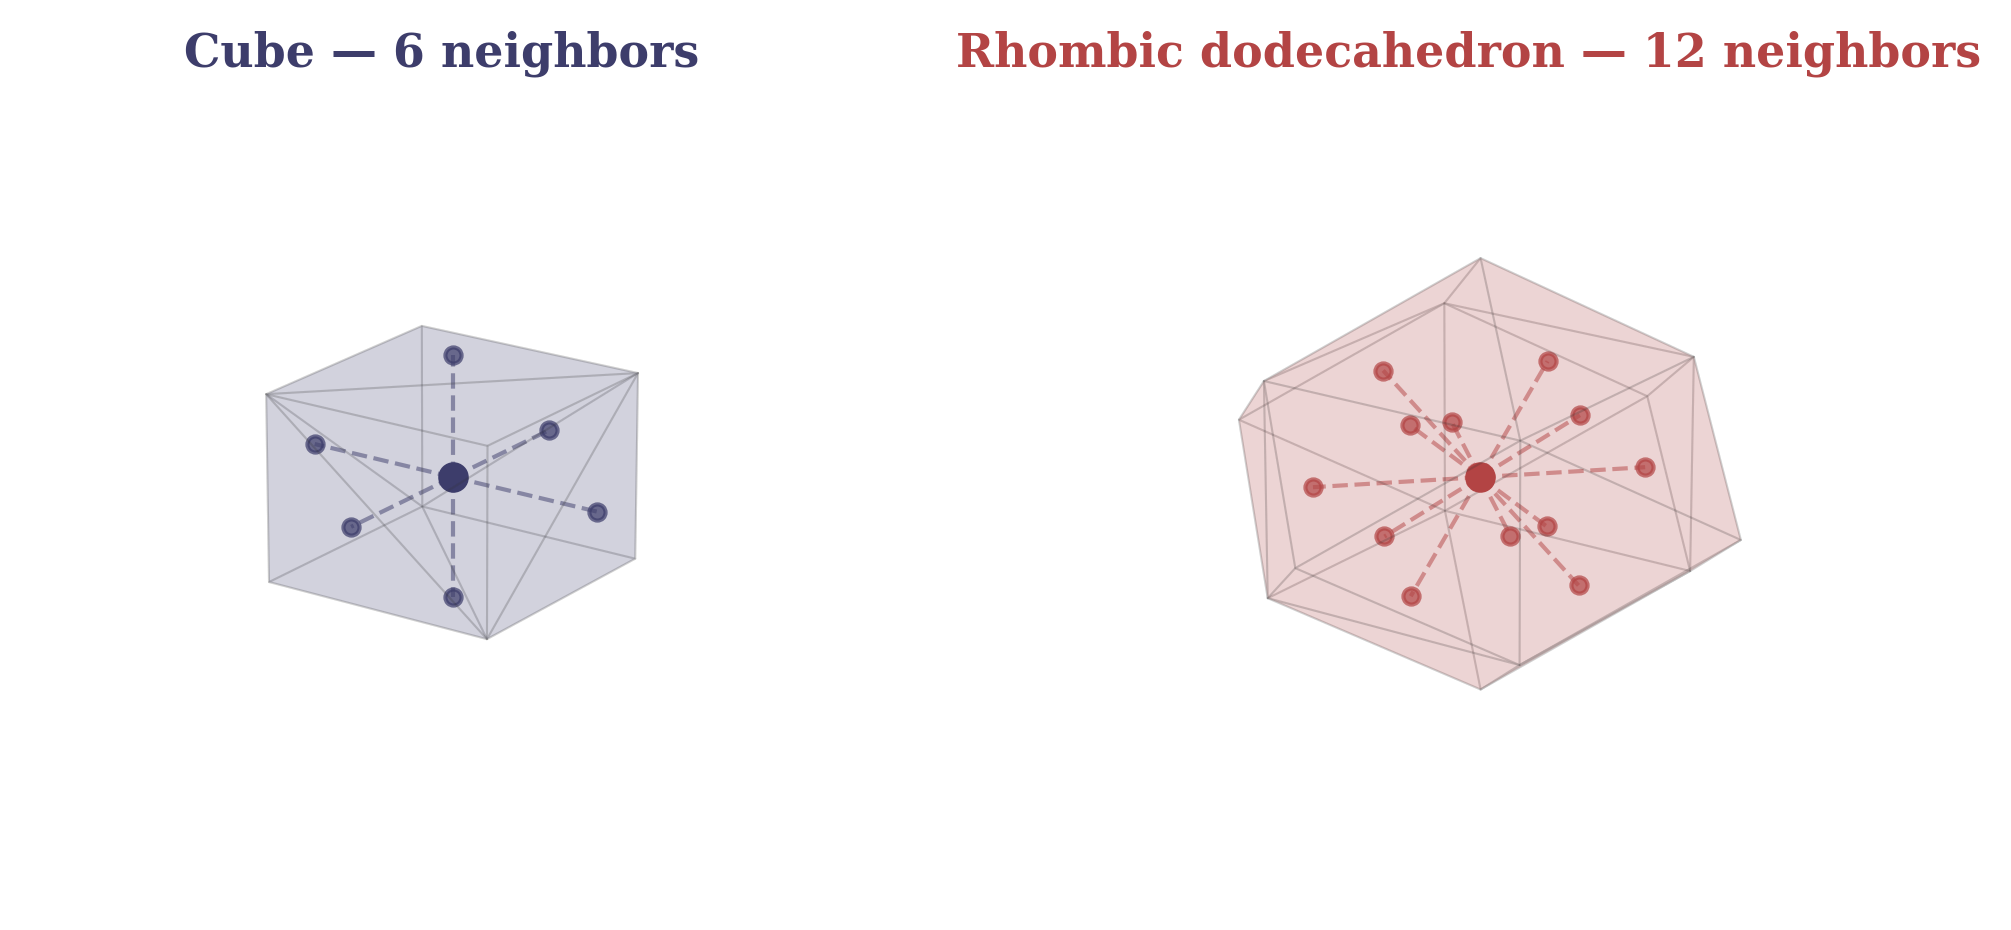
\includegraphics[width=\textwidth]{figures/fig1-voronoi-cells}
\caption{Voronoi cells of the SC and FCC lattices. Left: the cube
  (6 face-sharing neighbors along coordinate axes). Right: the
  rhombic dodecahedron (12 face-sharing neighbors spanning diagonal
  directions). Dashed lines indicate neighbor connectivity; dots mark
  neighbor positions.}
\label{fig:voronoi}
\end{figure}

\subsection{Sphere Packing and Signal Sampling}

Kepler conjectured (1611) that the FCC lattice achieves the densest
packing of equal spheres, with packing fraction
$\pi/(3\sqrt{2}) \approx 0.7405$. Both FCC and HCP (hexagonal
close-packed) achieve this density. Hales proved the conjecture
(published 2005~\cite{hales2005}; formally verified
2014--2017~\cite{hales2017}).

In 3D lattice sampling theory, optimality is formulated in the
reciprocal (frequency-domain) lattice. Petersen and
Middleton~\cite{petersen1962} established the general framework;
the commonly cited result in the volume-rendering literature
identifies the BCC lattice as the most efficient sampling geometry
for isotropic bandlimits, requiring ${\sim}29.3\%$ fewer samples
than SC at comparable fidelity~\cite{theussl2002orvs,theussl2001}.
The FCC and BCC lattices are reciprocal duals---their roles
reverse between real space and frequency space.

Our experiments evaluate FCC in the \emph{spatial} domain because
this work tests a single topology across all rungs (graph,
spatial, signal, and embedding), and FCC is the natural spatial
counterpart: it is the densest sphere packing, its Voronoi cell
(the rhombic dodecahedron) provides a highly isotropic space-filling
cell---its isoperimetric quotient exceeds that of the cube, and prior
work identifies FCC and BCC Voronoi cells as local maxima among
space-filling tessellations~\cite{conway1999}---and its 12-connected
graph structure produces the routing and propagation advantages
measured in Rungs~1--2. Rung~3 (Section~\ref{sec:signal})
directly measures FCC spatial sampling with a topology-agnostic
reconstructor, rather than deriving predictions from sampling
theory. A BCC baseline is a natural next control for isolating
sampling-theoretic contributions.

\subsection{Lattice Data Structures}

Practical adoption of non-cubic lattices remains limited.
Theu{\ss}l et al.~\cite{theussl2001} demonstrated FCC and BCC
voxelization for volume rendering. Csebfalvi~\cite{csebfalvi2010}
explored BCC sampling for medical imaging. Entezari et
al.~\cite{entezari2004} formalized FCC/BCC box splines for
signal reconstruction. However, no prior work presents a
systematic, multi-domain benchmark comparing SC and FCC topologies
at matched node counts with publicly available code.

% ===================================================================
\section{Methodology}
\label{sec:method}

\subsection{Lattice Construction}

Both lattices are constructed to fill a cubic bounding volume
with approximately matched node counts.

\textbf{Cubic lattice.} $n^3$ nodes placed at integer coordinates
$\{0, 1, \ldots, n{-}1\}^3$. Each interior node connects to its
6 face-sharing neighbors (von Neumann neighborhood). Edge count:
$3n^2(n-1)$.

\textbf{FCC lattice.} Nodes placed at $n^3$ SC positions plus
$3 \cdot n^2(n-1)$ face-center positions, yielding approximately
$4n^3$ total nodes\footnote{%
Exact count depends on boundary handling. We use
$\lfloor n/\sqrt[3]{4} \rfloor$ as the cubic side length to
achieve approximately $n$ FCC nodes.}. Each interior node connects
to its 12 nearest neighbors using the FCC neighbor offset vectors:
\begin{equation}
  \left\{\tfrac{1}{2}(\pm e_i \pm e_j) : 1 \leq i < j \leq 3\right\}
\end{equation}
yielding 12 edges per interior node.

\textbf{Matching.} For a target of $N$ nodes, we set
$n_{\mathrm{SC}} = \lfloor N^{1/3} \rfloor$ (yielding
$n_{\mathrm{SC}}^3$ SC nodes) and
$n_{\mathrm{FCC}} = \lfloor (N/4)^{1/3} \rfloor$ (yielding
${\sim}4 n_{\mathrm{FCC}}^3$ FCC nodes after deduplication).
The two counts are not identical---SC produces exact cubes while
FCC produces approximate counts---so we report exact node counts
alongside every metric. At all scales reported here, the counts
differ by less than 15\%.

\subsection{Software and Reproducibility}

All experiments use the \texttt{rhombic} library (Python 3.10+,
dependencies: NumPy, NetworkX, SciPy). Graphs are constructed as
NetworkX \texttt{Graph} objects. The complete benchmark suite is
reproduced via:
\begin{verbatim}
  pip install rhombic && python -m rhombic.benchmark
\end{verbatim}
Hardware: Windows 11, Intel CPU (graph/spatial benchmarks are
CPU-bound), NVIDIA RTX 6000 Ada 48\,GB (unused for these
benchmarks). Source code, raw data, and interactive demo are
publicly available (see Availability, Section~\ref{sec:conclusion}).

\paragraph{Reproducibility.}
All stochastic operations (signal evaluation points, embedding
generation, random node removal for fault tolerance) use a fixed
seed ($\mathtt{seed}=42$). Graph-theoretic benchmarks (Rung~1)
and spatial operations (Rung~2) are fully deterministic given the
lattice construction. Signal benchmarks (Rung~3) use a single
trial per frequency--scale combination with fixed evaluation
points. Embedding benchmarks (Rung~4) use a single trial with
fixed cluster generation. All results are reproduced by
\texttt{python~-m~rhombic.benchmark} from the \texttt{v0.1.2}
release (\texttt{pip install rhombic==0.1.2}). The PyPI artifact
includes provenance attestation linking the published package to
its source repository commit.\footnote{Cross-platform floating-point differences
may produce variations at the least-significant digit; all ratios
reported here are stable across tested platforms (Windows~11/Linux,
Python~3.10--3.12).}

% ===================================================================
% Transition: from geometric motivation to empirical measurement
\section{Rung 1: Graph Theory}
\label{sec:graph}

We now report empirical measurements: each rung defines a
matched-scale benchmark and reports observed benefit--cost ratios.

We measure four graph-theoretic properties at three scales
(125--4{,}000 nodes). All metrics are computed on the full
lattice graphs via NetworkX.

\subsection{Metrics}

\textbf{Average shortest path length} (ASPL): mean over all
node pairs, computed via BFS. \textbf{Diameter}: maximum
shortest path. \textbf{Algebraic connectivity}: second-smallest
eigenvalue of the graph Laplacian (Fiedler
value~\cite{fiedler1973}). \textbf{Fault tolerance}: fraction
of nodes reachable from the largest connected component after
removing 10\% of nodes uniformly at random.

\subsection{Results}

\begin{table}[H]
\centering
\caption{Graph theory benchmarks. All advantage ratios ${>}\,1$ indicate
FCC outperformance; edge ratio is cost.}
\label{tab:graph}
\begin{tabular}{lrrrrrr}
\toprule
Scale & Nodes (SC/FCC) & SC ASPL & ASPL$^a$ & Diam.$^a$
  & Alg.\ conn.$^b$ & Edge cost$^b$ \\
\midrule
${\sim}125$  & 125 / 108   & 4.84 & 1.45$\times$
  & 1.71$\times$ & 2.31$\times$ & 1.50$\times$ \\
${\sim}1000$ & 1000 / 864  & 9.91 & 1.46$\times$
  & 1.69$\times$ & 2.55$\times$ & 1.61$\times$ \\
${\sim}4000$ & 4096 / 4000 & 15.94 & 1.40$\times$
  & 1.61$\times$ & 2.43$\times$ & 1.88$\times$ \\
\bottomrule
\multicolumn{7}{l}{\footnotesize $^a$SC/FCC (shorter~=~better).
$^b$FCC/SC.}
\end{tabular}
\end{table}

The ASPL advantage is stable at 29--32\% across all scales
tested (Figure~\ref{fig:benchmarks}). The algebraic connectivity ratio (2.3--2.5$\times$)
exceeds the raw degree ratio (12/6 = 2$\times$), indicating
that the \emph{isotropy} of the FCC lattice~\cite{conway1999} compounds the
per-node connectivity advantage. The edge ratio approaches the
asymptotic limit of 2 as boundary effects diminish at larger
scales.

The path-length advantage has a geometric explanation: in a cubic
lattice, travel between non-axis-aligned points requires
axis-by-axis zig-zagging (the L1/Manhattan metric). FCC's diagonal
neighbors permit more direct routes, approaching the L2 (Euclidean)
distance. For a unit vector drawn uniformly on $S^2$, the expected
$\ell_1$ norm is $3/2$, so the mean $\ell_1/\ell_2$ ratio is
$3/2 = 1.50$, predicting a 33\% path-length reduction---consistent
with the observed 29--32\% (the gap likely reflecting finite-lattice
boundary effects).

\begin{figure}[t]
\centering
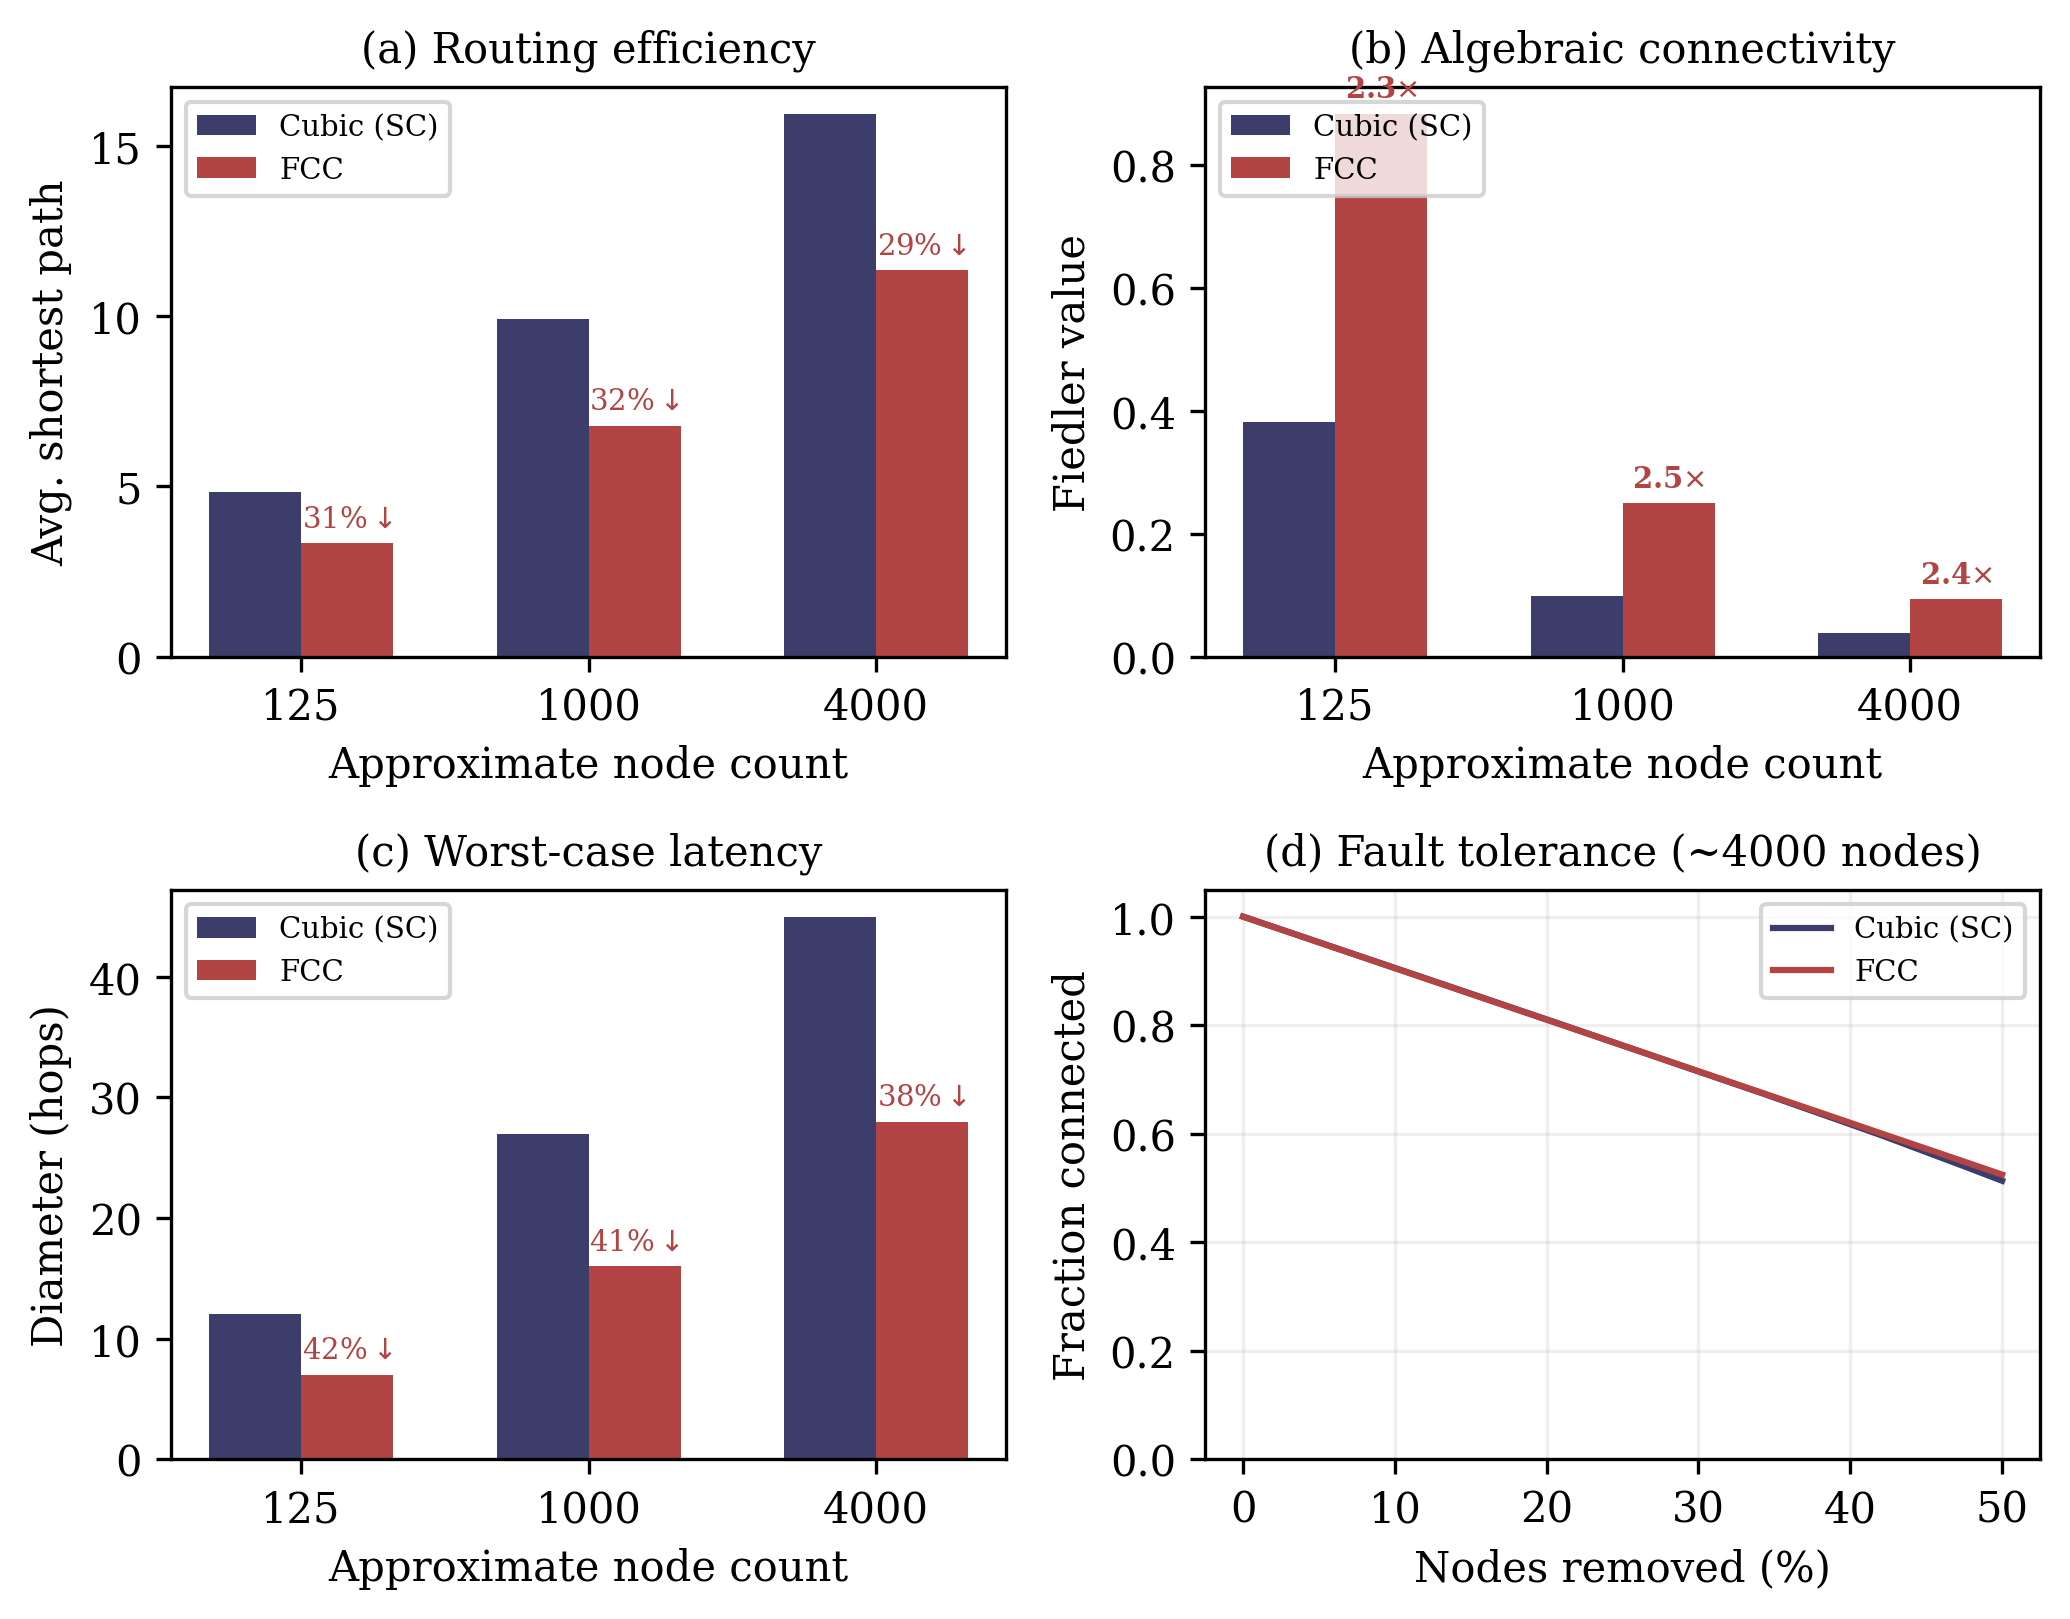
\includegraphics[width=\textwidth]{figures/fig2-graph-benchmarks}
\caption{Graph-theoretic benchmarks at matched scale. (a)~Average
  shortest path length: FCC reduces paths by 29--32\%. (b)~Algebraic
  connectivity (Fiedler value): FCC achieves 2.3--2.5$\times$ the
  cubic value. (c)~Diameter: FCC reduces worst-case latency by
  38--42\%. (d)~Fault tolerance at ${\sim}4{,}000$ nodes: fraction of
  the graph remaining connected as nodes are randomly removed.}
\label{fig:benchmarks}
\end{figure}

% ===================================================================
\section{Rung 2: Spatial Operations}
\label{sec:spatial}

Five spatial operations benchmarked at three scales (125--8{,}000
nodes). Lattice nodes serve as spatial data points; operations
use both graph structure and Euclidean coordinates.

\subsection{Operations}

\textbf{Nearest-neighbor query}: SciPy KDTree single-point query.
\textbf{Sphere/box range query}: all points within radius/box of
query point. \textbf{Flood fill}: BFS from a central node, counting
nodes reached at depth 3. \textbf{Spatial hash}: grid-based hash
with cell size $= 2 \times$ average nearest-neighbor distance.

\paragraph{Parameters.}
Sphere radius = 15\% of bounding-box diagonal, box extent = 30\%,
100 random queries per trial; reported timings exclude
tree-construction cost (included in the repository benchmarks).

\subsection{Results}

\begin{table}[H]
\centering
\caption{Spatial operations at ${\sim}8{,}000$ nodes
(SC: 8{,}000; FCC: 8{,}788).}
\label{tab:spatial}
\begin{tabular}{lrl}
\toprule
Operation & FCC vs.\ Cubic & Note \\
\midrule
\multicolumn{3}{l}{\textit{FCC advantages}} \\
Flood fill reach & $+55\%$ & More nodes per hop \\
NN query speed & $17\%$ faster & Denser packing, nearer neighbors \\
Spatial hash query & $6\%$ faster & Denser cells \\
Sphere query density & $+24\%$ nodes & More per volume \\
\midrule
\multicolumn{3}{l}{\textit{FCC costs}} \\
Range query time & $3$--$5\times$ slower & Density increases scan work \\
\bottomrule
\end{tabular}
\end{table}

The results reveal a clear decision boundary:
\textbf{propagation-dominated} workloads (flood fill, wavefront
expansion, influence spreading) benefit unambiguously from FCC.
\textbf{Enumeration-dominated} workloads (range queries that scan
all nodes in a volume) pay a density cost proportional to the
packing efficiency. Point queries (NN, hash lookup) favor FCC
due to denser packing producing nearer nearest neighbors.

% ===================================================================
\section{Rung 3: Signal Processing}
\label{sec:signal}

\subsection{Method}

Both lattices fill $[0,1]^3$ with density-matched sample counts.
An isotropic test signal
\begin{equation}
  f(\mathbf{x}) = \sin(\omega x)\cos(\omega y)\sin(\omega z)
    + 0.5\cos(\omega r) + 0.3\sin\!\left(\omega\tfrac{x+y+z}{\sqrt{3}}\right)
\end{equation}
where $r = \|\mathbf{x}\|$ and $\omega = 2\pi f$, is sampled at
lattice nodes and reconstructed at 600--800 random evaluation points
via thin-plate-spline RBF interpolation (SciPy, zero smoothing).
Frequencies sweep from 10\% to 100\% of the cubic Nyquist frequency.

\subsection{Results}

\begin{table}[H]
\centering
\caption{Signal reconstruction: peak FCC advantage in the
productive frequency range (10--60\% of Nyquist).}
\label{tab:signal}
\begin{tabular}{rrrr}
\toprule
Samples & Peak $\Delta$PSNR & Best MSE ratio & Isotropy ratio \\
\midrule
216   & $+6.1$ dB  & $4.2\times$ & $0.20\times$ \\
512   & $+7.3$ dB  & $5.3\times$ & $0.05\times$ \\
1{,}000 & $+10.0$ dB & $10\times$  & $0.11\times$ \\
\bottomrule
\end{tabular}
\end{table}

The advantage \emph{grows with scale} because the geometric
Nyquist region advantage has more ``room'' to express itself at
higher sample densities. Above the Nyquist limit, both lattices
alias and we observe cases where axis alignment in the cubic lattice
reduces error for separable signal components. We treat this as an
axis-alignment artifact rather than a general advantage.

The isotropy metric (directional variance of reconstruction error)
shows that FCC reconstruction error is 5--20$\times$ more uniform
across directions. These are direct empirical measurements using a
topology-agnostic reconstructor, not derivations from sampling
theory. This measurement approach---comparing directional error
variance rather than aggregate error alone---may be useful for
evaluating lattice quality independent of the FCC argument.

% ===================================================================
\section{Rung 4: Embedding Neighborhood Preservation}
\label{sec:embed}

\subsection{Method}

We generate 125--1{,}000 clustered embeddings in 128 dimensions
(5 Gaussian clusters with overlap). Embeddings are projected to 3D
via random orthogonal projection (chosen to avoid bias from any
particular axis alignment) and assigned to lattice nodes via
KDTree nearest-assignment. Three benchmarks measure how well the
lattice topology preserves high-dimensional neighborhood structure.

\textbf{Neighborhood recall}: fraction of an embedding's true 10
nearest neighbors (brute-force in 128D) captured by its lattice
node's $k$-hop neighborhood. \textbf{Information diffusion}: rounds
for a signal pulse to reach 50\%/80\% of the lattice.
\textbf{Consensus}: Laplacian averaging rounds to convergence
($\epsilon = 0.05$).

\subsection{Results}

\begin{table}[H]
\centering
\caption{Neighborhood recall at 1-hop and 2-hop.}
\label{tab:recall}
\begin{tabular}{rrrrr}
\toprule
Nodes (SC/FCC) & SC 1-hop & FCC 1-hop & SC 2-hop & FCC 2-hop \\
\midrule
125 / 108   & 0.641 & \textbf{0.903} & 0.932 & \textbf{0.998} \\
512 / 500   & 0.547 & \textbf{0.763} & 0.840 & \textbf{0.971} \\
1000 / 864  & 0.508 & \textbf{0.658} & 0.756 & \textbf{0.915} \\
\bottomrule
\end{tabular}
\end{table}

At 1-hop, FCC captures 15--26 more percentage points of true
nearest neighbors. Information diffuses 1.4--2$\times$ faster.
Consensus converges 1.58$\times$ faster at 500 nodes, though
per-neighbor weight dilution ($1/13$ vs.\ $1/7$) reduces the
advantage at 1{,}000 nodes (0.93$\times$).

% ===================================================================
\section{FCC Embedding Index}
\label{sec:index}

To test whether the topology advantage survives a realistic
retrieval workload, we implement a proof-of-concept ANN index.

\subsection{Architecture}

\begin{enumerate}
  \item \textbf{Project} embeddings from $d$ dimensions to 3D via
    PCA (deterministic, preserves maximum variance). PCA is used
    here, rather than the randomized projection of Rung~4, because a
    practical retrieval pipeline would typically project along
    maximum-variance directions. (PCA is linear; nonlinear projections
    might yield different absolute recall, but the topology comparison
    remains valid because both lattices receive identical embeddings.)
  \item \textbf{Quantize} to lattice nodes via KDTree
    nearest-assignment.
  \item \textbf{Store} original $d$-dimensional vectors at their
    assigned nodes.
  \item \textbf{Query} by projecting the query to 3D, finding its
    lattice node, collecting all vectors from the $k$-hop
    neighborhood, and ranking by cosine similarity in the original
    space.
\end{enumerate}

Both \texttt{FCCIndex} and \texttt{CubicIndex} share the same
\texttt{LatticeIndex} base class. The architectural difference between them is the
connectivity pattern (though actual node counts also differ slightly;
Table~\ref{tab:index}).

\subsection{Results}

\begin{table}[H]
\centering
\caption{Recall@10 on synthetic embeddings (384D, 30 overlapping
clusters, 1{,}800 corpus vectors, 200 queries). Ground truth by
brute-force cosine similarity.}
\label{tab:index}
\begin{tabular}{rllrrr}
\toprule
Target & Topology & Actual & 1-hop & 2-hop & 3-hop \\
\midrule
125  & Cubic       & 125 & 0.379 & 0.788 & 0.999 \\
125  & \textbf{FCC}& 108 & \textbf{0.445} & \textbf{0.971} & \textbf{1.000} \\
\midrule
500  & Cubic       & 512 & 0.085 & 0.324 & 0.551 \\
500  & \textbf{FCC}& 500 & \textbf{0.280} & \textbf{0.488} & \textbf{0.789} \\
\midrule
1000 & Cubic       & 1000 & 0.044 & 0.138 & 0.414 \\
1000 & \textbf{FCC}& 864 & \textbf{0.216} & \textbf{0.349} & \textbf{0.616} \\
\bottomrule
\end{tabular}
\end{table}

The FCC index achieves +7 to +20 percentage points higher recall
at 1-hop across all scales. At 500 target nodes, the gap is
largest: 28.0\% vs.\ 8.5\%, a 3.3$\times$ relative improvement.
The advantage is consistent with the connectivity difference, since the
projection, assignment, and ranking procedures are identical. However,
node-count mismatch (Table~\ref{tab:index}) may also contribute; a
matched-count control is noted as future work. The FCC advantage is
consistent across both projection methods (random orthogonal in
Rung~4, PCA in Section~\ref{sec:index}), suggesting the topology
effect is robust to projection choice.

% ===================================================================
\section{Discussion}
\label{sec:discussion}

\subsection{The Pattern}

The following interpretations are consistent with the measurements
above; they are hypotheses about mechanism, not proofs of causality.

Across all four domains, a consistent pattern emerges:

\textbf{Propagation wins.} Any workload where information spreads
through the lattice---routing, flooding, diffusion, signal
reconstruction, neighbor retrieval---benefits from FCC topology.
The 12-connected structure propagates faster, farther, and more
isotropically than 6-connected.

\textbf{Isotropy wins.} The FCC lattice's 12 neighbors span
directions uniformly. The cubic lattice's 6 neighbors span only
coordinate axes. For tasks without a preferred direction (embedding
similarity, signal bandwidth, fault propagation), isotropy is the
superior geometry.

\textbf{Enumeration pays.} Range queries that must scan all nodes
in a region pay a density cost proportional to the packing
efficiency (${\sim}1.24\times$ more nodes per volume, scanned
$3$--$5\times$ more slowly).

\subsection{Scale Invariance}

The ratios reported in Sections~\ref{sec:graph}--\ref{sec:embed}
are stable across all scales tested (125--8{,}000 nodes). This
stability suggests a geometric origin: at scales well above the
boundary layer, the ratios are determined by the coordination number
(12 vs.\ 6), the kissing number configuration, and the Voronoi cell
shape---constants of the lattice, not functions of sample size. Whether
this stability extends to scales beyond those tested here is an
empirical question for future work.

\subsection{The Cost}

The FCC lattice uses approximately $2\times$ more edges than the
SC lattice at matched node counts (asymptotically exact: $12/6 = 2$).
Table~\ref{tab:cost} contextualizes this cost across domains.

\begin{table}[H]
\centering
\caption{Cost of $2\times$ edges in different domains.}
\label{tab:cost}
\begin{tabular}{lll}
\toprule
Domain & Edge cost & $2\times$ edges means \\
\midrule
Physical network & Wire, trace, power & Real constraint \\
Software structure & 8-byte pointer & ${\sim}$96 vs.\ 48 bytes/node \\
Logical topology & Nothing until traversed & Arrive 30\% sooner \\
Embedding index & One candidate to evaluate & +7--20pp recall \\
Signal sampling & One measurement & 5--10$\times$ better fidelity \\
\bottomrule
\end{tabular}
\end{table}

The domains where the cost is prohibitive (chip interconnect) are
those where the advantage matters most. The domains where the cost
is trivial (software, logical topology) are those where adoption is
easiest.

\subsection{Cybernetic Interpretation}

The following connections are interpretive, not empirical; they
suggest why the measured advantages arise but do not constitute
independent evidence.

Ashby's Law of Requisite Variety~\cite{ashby1956} predicts the
algebraic connectivity result: a system must match the variety of
perturbations it faces. A 12-connected cell absorbs perturbation
along 12 directions; the isotropy compounds beyond the raw $2\times$
degree ratio to produce $2.3$--$2.5\times$ algebraic connectivity.
Beer's Viable System Model~\cite{beer1972} distinguishes fragile
hierarchies (easily partitioned along axes) from viable systems
(redundant paths resist fragmentation). The SC lattice is axis-aligned
and axis-fragile; the FCC lattice is isotropic and robust.

\subsection{When the Cubic Lattice Wins}

The SC lattice retains practical advantages in several scenarios.
\textbf{Memory layout:} cubic addressing maps directly to linear
memory via $i + jN + kN^2$, enabling SIMD vectorization and
cache-line-aligned access patterns that FCC addressing disrupts.
\textbf{Range queries:} at 8{,}000 nodes, sphere and box queries
run 3--5$\times$ slower on FCC (Table~\ref{tab:spatial}) because
denser packing produces more candidates to scan.
\textbf{Consensus at scale:} Laplacian averaging on FCC converges
slower than SC at 1{,}000 nodes (0.93$\times$) due to per-neighbor
weight dilution ($1/13$ vs.\ $1/7$).
\textbf{Axis-aligned workloads:} when the signal or access pattern
is inherently axis-aligned (separable filters, rectilinear scans),
the SC lattice's coordinate alignment is an advantage, not a
limitation.

\subsection{Limitations and Threats to Validity}

\textbf{Three dimensions only.} These results are specific to 3D
lattices. Extension to higher dimensions (D$_4$ in 4D, $E_8$ in
8D, Leech lattice in 24D) is future work.

\textbf{Proof-of-concept index.} The FCC embedding index is not
competitive with production ANN systems (HNSW, IVF-PQ). It exists
to isolate the topology variable, not to propose a deployment
architecture.

\textbf{No formal null model.} We compare FCC to SC directly. A
formal analysis decomposing the advantage into degree-attributable
and isotropy-attributable components would strengthen the
theoretical contribution.

\textbf{Targeted fault tolerance.} We tested random node removal.
Under targeted attack (removing high-betweenness nodes), the FCC
advantage should be more dramatic.

\textbf{Single-trial benchmarks.} Signal and embedding benchmarks
use a single trial per configuration with a fixed seed. While the
deterministic results are exactly reproducible, confidence
intervals from multiple seeds would strengthen statistical claims.

\textbf{Scale range.} All benchmarks operate between 125 and
8{,}000 nodes. The stability of ratios across this range is
consistent with geometric origin, but extrapolation beyond tested
scales is not empirically verified.

% ===================================================================
\section{Conclusion}
\label{sec:conclusion}

For the isotropic, propagation-dominated workloads tested here, the
SC lattice is consistently outperformed. Across four independent
domains and five experimental rungs, the FCC lattice provides
measurable, reproducible advantages that are stable across all
tested scales. The cost is bounded (${\sim}2\times$ edges) and
the benefit compounds (30\% routing $+$ 55\% propagation $+$
5--10$\times$ signal fidelity $+$ 15--26pp neighborhood recall).

The FCC lattice (with HCP) achieves the densest sphere packing and
the topology that close-packed natural structures commonly exhibit. The SC
lattice persists in computation largely through convention rather than
demonstrated optimality for isotropic workloads. This
library and this paper provide the quantitative basis for
reconsidering that inheritance. For practitioners evaluating lattice
topology in their own domains, we recommend measuring directly:
\texttt{pip install rhombic \&\& python -m rhombic.benchmark}.

\paragraph{Availability.}
Source code: \url{https://github.com/promptcrafted/rhombic}.\\
Package: \url{https://pypi.org/project/rhombic/}.\\
Interactive demo: \url{https://huggingface.co/spaces/timotheospaul/rhombic}.

% ===================================================================
\section*{Acknowledgments}

The author thanks Araminta K for partnership in Promptcrafted, and
the cybernetics of Ashby, Beer, and Bateson for the interpretive
framework. Portions of the codebase and manuscript were developed
with AI assistance (Claude, Anthropic).

% ===================================================================
\bibliographystyle{plainnat}
\bibliography{rhombic}

\end{document}
